%%%%%%%%%%%%%%%%%%%%%%%%%%%%%%%%%%%%%%%%%%%%%%%%%%%%%%%%%%%%%%%
%
% Welcome to writeLaTeX --- just edit your LaTeX on the left,
% and we'll compile it for you on the right. If you give 
% someone the link to this page, they can edit at the same
% time. See the help menu above for more info. Enjoy!
%
%%%%%%%%%%%%%%%%%%%%%%%%%%%%%%%%%%%%%%%%%%%%%%%%%%%%%%%%%%%%%%%
%
% For more detailed article preparation guidelines, please see:
% http://f1000research.com/author-guidelines

%\title{BioJS InterMine List Analysis}

\documentclass[10pt,a4paper,twocolumn]{article}

\usepackage{f1000_styles}
\usepackage{listings}
\usepackage[colorlinks]{hyperref}
\usepackage{url}
\usepackage{appendix}

\definecolor{dkgreen}{rgb}{0,0.6,0}
\definecolor{gray}{rgb}{0.5,0.5,0.5}
\definecolor{mauve}{rgb}{0.58,0,0.82}

\lstdefinelanguage{JavaScript}{
  keywords={typeof, new, true, false, catch, function, return, null, catch, switch, var, if, in, while, do, else, case, break},
  keywordstyle=\color{blue}\bfseries,
  ndkeywords={class, export, boolean, throw, implements, import, this},
  ndkeywordstyle=\color{darkgray}\bfseries,
  identifierstyle=\color{black},
  sensitive=false,
  comment=[l]{//},
  morecomment=[s]{/*}{*/},
  commentstyle=\color{purple}\ttfamily,
  stringstyle=\color{red}\ttfamily,
  morestring=[b]',
  morestring=[b]"
}

\lstset{frame=tb,
  language=JavaScript,
  aboveskip=3mm,
  belowskip=3mm,
  showstringspaces=false, columns=flexible,
  basicstyle={\small\ttfamily},
  numbers=none,
  numberstyle=\tiny\color{gray},
  keywordstyle=\color{blue},
  commentstyle=\color{dkgreen},
  stringstyle=\color{mauve},
  breaklines=true,
  breakatwhitespace=true
  tabsize=3
}

\begin{document}

\title{\textit{BioJS} InterMine List Analysis:
A BioJS component for displaying graphical or statistical analysis of
collections of items from InterMine web-service endpoint.
}

\author[1]{Radek Štěpán \thanks{radek@intermine.org}}
\author[1]{Alexis Kalderimis \thanks{alex@intermine.org}}
\author[1]{Julie Sullivan \thanks{julie@flymine.org}}
\author[1]{Rachel Lyne \thanks{rachel@flymine.org}}
\author[1]{Michael Lyne \thanks{mike@intermine.org}}
\author[1]{Gos Micklem \thanks{g.micklem@gen.cam.ac.uk - corresponding author}}
\affil[1]{
    Department of Genetics and Cambridge Systems Biology Centre,
    Cambridge University, Downing Street, Cambridge, CB2 3EH, UK.
}

\maketitle
\thispagestyle{fancy}

\begin{abstract}

\textbf{Summary:}
We describe a reusable BioJS JavaScript component for the display of list
analysis results from InterMine compatible web-services. This component can display
statistical and graphical analyses of a user-defined collection of entities stored
in a data warehouse. We explain how to instantiate and use this component, and
define the potential benefits to the bioinformatics web-development community.

\textbf{Availability:}
\href{https://github.com/alexkalderimis/im-widgets-biojs} and
\href{http://github.com/biojs/biojs}

\textbf{Contact:} g.micklem@cam.ac.uk

\end{abstract}
\clearpage

\section*{Introduction}

InterMine~\cite{intermine} is a platform for building data warehouses which
includes specialisations for the life-sciences. As part of the
InterMOD~\cite{intermod} project, a number of InterMine data-warehouses have
been developed and released to the public containing high-quality integrated
data curated by the major model organism database (MOD) organisations. In
addition, the InterMine platform is widely used by other projects, such as the
modENCODE project~\cite{contrino2012}, as well as a range of other resources
including metabolicMine~\cite{metabolicmine}, TargetMine~\cite{targetmine},
FlyTFMine~\cite{flytfmine}, and MitoMiner~\cite{mitominer}. This means that
reliable integrated data sets exist for use by researchers working in a wide
range of fields in the life-sciences, which can be accessed by a common
interface.

One of the features of the InterMine system is the ability to store named sets
of entities, called \emph{lists}, and refer to them in queries and other
analysis. This allows a user, for example, to save a list of genes and reuse
this saved collection easily. The InterMine system also allows specialised
analysis to be performed taking advantage of the integrated nature of the data
warehouse system. For example the system can run queries that aggregate
information about relationships between data types, and provide indications of
levels of statistical significance for the results (\emph{enrichment queries}).

Until recently, the output of these list analysis tools was only accessible
through the web-application built into the InterMine system. Recent work on the
InterMine web-services has enabled this functionality to be externalised into
the list-widgets~\cite{site:list-widgets} project: separate JavaScript based
components that can be used in third party web-sites.  These developments have
already been incorporated into the standard InterMine web-application
configuration, meaning that users of the tools described here have access to the
same query and display mechanisms in their own sites that are available through
the standard InterMine web-application.

InterMine supports the aims of the BioJS~\cite{biojs} initiative to provide
well-designed, robust web-site components to application developers in order to
foster code reuse and minimise duplicated effort. This leads us to contribute to
the BioJS project this set of components for running list analysis tools and
displaying their output, so that they may be widely distributed, and
interoperate with tools from other developers.

\subsection*{Installation}

As a JavaScript web component, these tools are designed to be run within the
JavaScript virtual machines provided by modern browsers, and render to HTML
pages. Installation means indicating to the remote client (the user), which
resources to load as dependencies, as well as where these are located. Typically
this is done by adding references to these resources in the \texttt{head}
section of a page through the use of \texttt{script} element (see code
sample~\ref{code:loading}). Recent practice suggests loading these resources in
at the end of the \texttt{body} improves page load time. The dependencies that
must be loaded to use these tools are listed in appendix~\ref{app:deps}.

The BioJS InterMine list analysis library needs to be downloaded from the BioJS
registry~\cite{site:biojs-registry} and hosted in an accessible location.

\begin{lstlisting}[caption={Loading the list analysis tools library.}, label={code:loading}]
<script src="Biojs.InterMine.ListAnalysis.js"></script>
\end{lstlisting}

\subsection*{Usage}

Once the BioJS component and its dependencies are loaded, the component itself
may be instantiated, which creates a new list analysis displayer, inserts it
into the document, and populates it with the appropriate data by calling to the
InterMine web-services. This requires that an element exist within the document
(see code listing~\ref{code:div}) into which the component can be inserted.

\begin{lstlisting}[caption={The target document element},label={code:div}]
<div id="list-analysis-example"></div>
\end{lstlisting}

The JavaScript code to instantiate the component refers to this element as the
\texttt{target}, and provides the other arguments required to specify which
\texttt{list} we wish to analyse, the \texttt{url} of the service where that
list is to be found, and which specific analysis \texttt{tool} we wish to run.
The example below uses a list of genes encoding putative \emph{D. melanogaster}
transcription factors made available as a public list at FlyMine~\cite{flymine}
and runs the pathway enrichment statistical analysis tool. The full list of
available lists (which each user can extend by creating personal lists) and
analysis tools can be accessed from the InterMine service being used.

\subsection*{Relationship Enrichment}

One category of tools is the \emph{enrichment tools}, which run queries that
attempt to find relationships that are statistically significant for the set of
entities as a whole.  For example, FlyMine~\cite{flymine} contains both genes,
loaded from sources such as FlyBase~\cite{flybase}, and biochemical pathways,
loaded from sources such as KEGG~\cite{kegg} and Reactome~\cite{reactome}.  The
pathways enrichment tool lists pathways of which genes in the list are members,
ordered by the degree of significance for the list of genes as a whole.

For example, if one gene in a list is in a particular pathway, but none of the
others are, it would be considered less significant than a pathway that all or
most genes in a list belonged to. Similarly, the background probability that a
particular relationship exists for an item is taken into account, meaning for
example that finding a publication that lists many or even all genes for a
organism, such as Clark 2007~\cite{Clark:2007}, would not be considered as
significant as a publication that mentions fewer genes, but with most of them
being in the list of interest.

The p-values used as measures of statistical significance are calculated by
modelling the relationships as a hypergeometric distribution (as Rivals
2007~\cite{rivals} and Beissbarth 2004~\cite{beissbarth}), which determines the
probability that a relationship between two entities would be selected at random
given the set of items to choose from. Let $n$ be the number of items in the
list, and $N$ be the size of the reference population, and $k$ be the number of
items in the list which are involved in the given relationship (are mentioned in
the publication, for example, or belong to a particular biochemical pathway),
and $M$ be the number of items in the reference population which share that
same relationship. Then for each relationship

$$P = \frac{{M \choose k} {N-M \choose n-k}}{{N \choose n}}$$
      
The options made available for multiple test correction include the Bonferroni,
Holm-Bonferroni, and Benjamini Hochberg~\cite{benjamini} algorithms.

The tools in this category are all prefixed with \texttt{enrichment:}, and can
be loaded as follows:

\begin{lstlisting}[caption={Loading an enrichment list analysis tool.},label={code:load-enrichment}]
var ListAnalysis = Biojs.InterMine.ListAnalysis;
var analysis = new ListAnalysis({
  target: "list-analysis-example",
  url: "http://www.flymine.org/query",
  list: "PL FlyTF_putativeTFs",
  tool: "enrichment:pathway_enrichment"
});
\end{lstlisting}

Once run, the component should be inserted into the document (see
Figure~\ref{fig:pathways}). The
component allows the user to adjust the parameters of the analysis, including the multiple
test correction method used, the p-value threshold and the background population.

\begin{figure}[htbp]
\centering
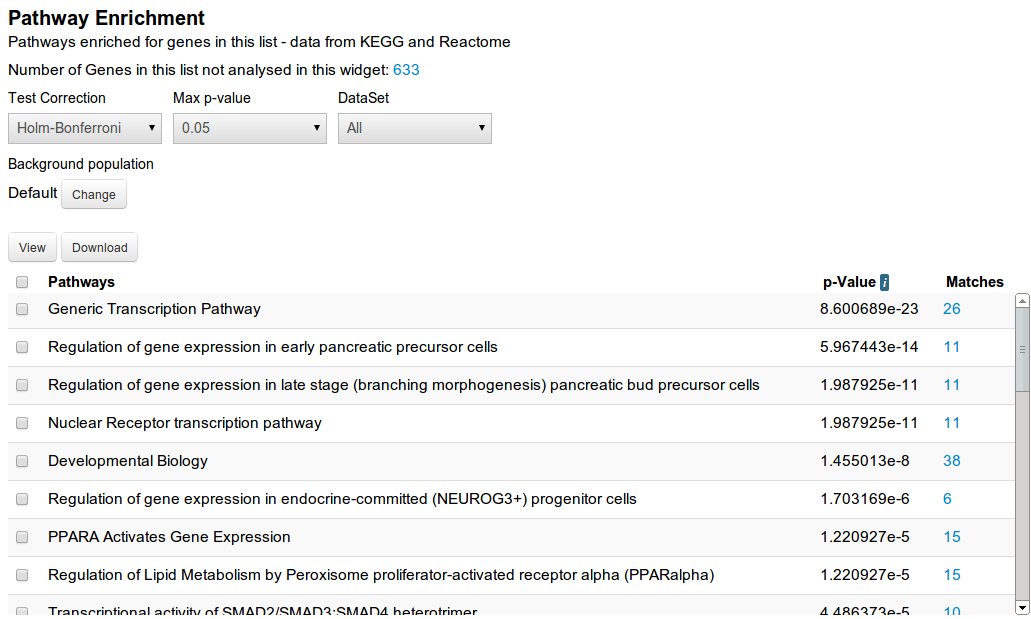
\includegraphics[width=0.4\textwidth]{pathway-enrichment.png}
\caption{\label{fig:pathways}A list analysis tool displaying the results of a
statistical analysis query.}
\end{figure}

\begin{figure}[hbp]
\centering
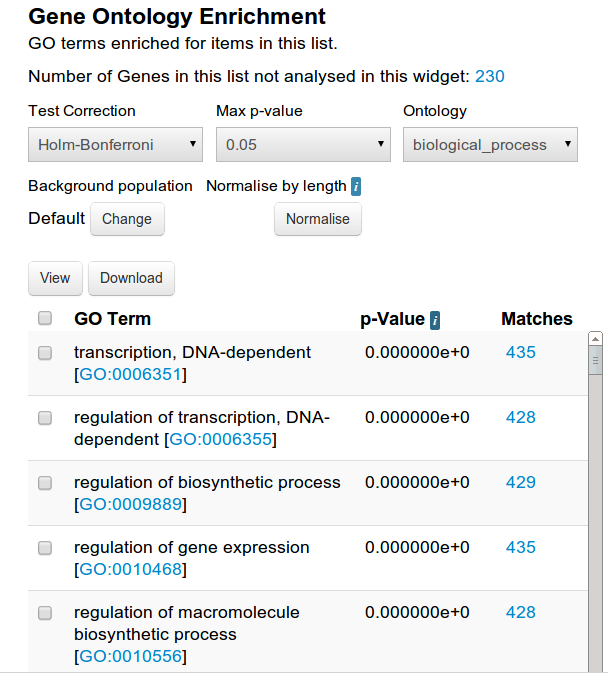
\includegraphics[width=0.4\textwidth]{go-enrichment.png}
\caption{\label{fig:go-enrichment}A list analysis tool displaying the results of the Gene Ontology (GO)
statistical analysis query.}
\end{figure}

The component also allows the user to interact with the results in a number of
ways, specifically: by clicking on an individual item that was matched; by
clicking on a button to show a set of matches; and by clicking on a button to
request that the selected items be saved to some location.  All these actions
cause the component to emit events, which can be listened for and handled by the
host JavaScript application. For example, to alert a string such as \texttt{Gene
- FGBN0123} when a user clicks on the corresponding element, one might attach an
event listener to capture the \texttt{onClickMatch} event, see code
listing~\ref{code:event-listener}.

\begin{lstlisting}[caption={Listening for a click event.}, label={code:event-listener}]
analysis.onClickMatch(function (ident, type) {
  alert(type + " - " + ident);
});
\end{lstlisting}

This enables the behaviour of the component to be integrated into
the hosting application. The full listing of events and their arguments is
included in the BioJS API documentation~\cite{site:biojs-doc}.

The canonical example for the use of statistical enrichment in bioinformatics is
enrichment of Gene Ontology (GO) terms for sequence annotations (Rivals
2007~\cite{rivals}). This functionality is supported as one of the statistical
analysis tools (see Figure~\ref{fig:go-enrichment}), within this more generic
enrichment analysis framework. The GO enrichment tool merits some further notes,
however, as it supports some of the more advanced parameters.

The GO enrichment tool demonstrates the use of optional filter parameters to
limit the results in some way. In the GO tool, it allows the user to select the
sub-ontology they are interested in. The user can also choose to normalise the
results of this tool, in this case by transcript length. 
% TODO: describe length normalisation.

\subsection*{Charts}

The other main category of analysis tools is the \emph{chart tools}. These run
aggregate queries over the items in a list, and present the information
graphically in interactive charts. The InterMine system supports both numerical
and categorical charting, reflected in the supported chart formats: bar charts,
line charts, pie charts and scatterplots.

Loading a chart analysis tool is identical to loading a statistical enrichment
tool - only the name of the tool need differ (see code
listing~\ref{code:load-chart}).

\begin{figure}
\centering
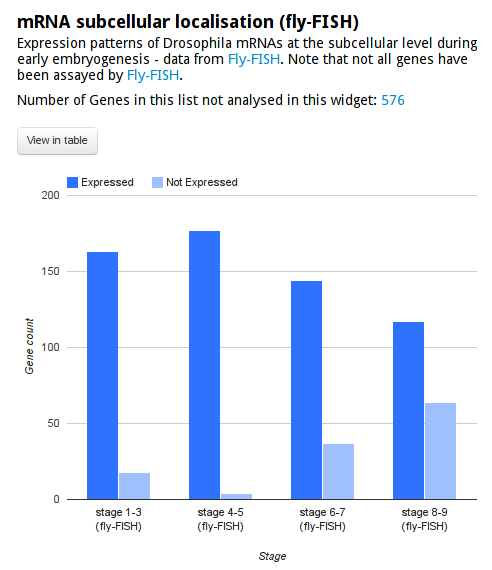
\includegraphics[width=0.4\textwidth]{im-widgets-flyfish.png}
\caption{
    \label{fig:flyfish}
    A list analysis component displaying the results of a the \texttt{chart:flyfish}
    tool (loaded in Code Listing ~\ref{code:load-chart}), which queries against
    Fly-FISH~\cite{flyfish} data.
}
\end{figure}

\begin{lstlisting}[caption={Loading a chart list analysis tool.},label={code:load-chart}]
var chart = new Biojs.InterMine.ListAnalysis({
  target: "list-analysis-example",
  url: "http://www.flymine.org/query",
  list: "PL FlyTF_putativeTFs",
  tool: "chart:flyfish"
});
\end{lstlisting}

This code will request data for the particular tool (\texttt{flyfish}), as run
against the given input list (\texttt{PL FlyTF\_putativeTFs}), and then display
the results in the appropriate chart format (Figure ~\ref{fig:flyfish}). The
chart tools have fewer parameters; they may take a single parameter, as detailed
in the tool description available from the relevant service (e.g.
\texttt{http://www.flymine.org/query/service/widgets}).

\begin{figure}
\centering
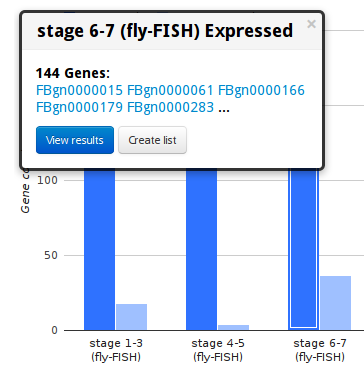
\includegraphics[width=0.4\textwidth]{im-widgets-flyfish-selected.png}
\caption{\label{fig:click-chart}The result of a user clicking on the
\emph{"stage 6-7, expressed"} bar of the chart.}
\end{figure}

In most cases they do not provide mechanisms for the user to change the results
displayed. They do however provide several mechanisms for the user to interact
with the results displayed. The user can click on the groupings or data-points
represented on the chart (see Figure ~\ref{fig:click-chart}), which allows the
user to trigger the same events available to enrichment tools, which can be
captured the same way (see code listing~\ref{code:event-listener}).

\section*{Discussion}

This tool addresses an important set of needs for bioinformatics developers: the
ability to perform enrichment analysis, and the the visualisation of typed
relationships between entities.  The InterMine platform, and this BioJS
component make performing these analyses and displaying the output
straightforward. It allows the developers to focus on integrating this
functionality where it is needed, and users to focus on interpreting rather than
retrieving the data. It is expected that wide availability of these tools will
provide significant savings in time for typically stretched developers and
researchers.  By providing this functionality as a BioJS component, it is hoped
that integration between different tools will result in the creation of
applications that are able to integrate analysis and visualisation from
different platforms.

\section*{Conclusions}

It is hoped that this component will prove useful to those developing tools for
researchers in the life-sciences. Significant work has gone into creating,
curating and combining high quality data sets. The recent work in exposing these
resources through web-services and producing reusable web-based components
allows this investment to benefit not just visitors to sites based on InterMine
applications, but any developer or user who aims to include this kind of
statistical analysis and visualisation in their platform. By providing
bioinformatics web-developers, and their users, with access to a broad range of
data sources meeting the needs of many diverse research communities, we
expect to help reduce the development burden on projects with limited resources,
and help minimise redundancy of effort.

\subsection*{Author contributions}

Alex Kalderimis wrote the manuscript and implemented the BioJS wrapper, under
the supervision of Gos Micklem, to a set of user specifications supplied by
Julie Sullivan, with feedback given by Rachel Lyne, Radek Štěpán and Mike Lyne.
Radek Štěpán implemented the list analysis component.

\subsection*{Acknowledgements}
The author thanks Manuel Corpas for useful feedback.

\subsection*{Competing interests}

The authors declare that there are no competing interests.

\subsection*{Grant information}
InterMine has been developed with the support of the following grants, awarded
to Dr. G. Micklem.

\begin{enumerate}
\item the Wellcome Trust
 \begin{itemize}
 \item{Grant number: 090297}
 \end{itemize}
\item and the National Human Genome Research Institute.
 \begin{itemize}
 \item{Grant number: R01HG004834}
 \end{itemize}
\end{enumerate}

The content is solely the responsibility of the authors and does not necessarily
represent the official views of the funding bodies.

\nocite{*}
{\small\bibliographystyle{unsrt}
\bibliography{references}}

\section*{Appendix}
\appendix
\section{Dependencies} \label{app:deps}

\lstset{language=HTML}

% Have to manually break the URLs or else
% they overflow.
\begin{lstlisting}
<link rel="stylesheet" type="text/css"
      href="http://cdn.intermine.org/
js/intermine/apps-c/list-widgets/2.0.
4/app.bundle.prefixed.min.css">
<script src="http://cdn.intermine.org
/js/intermine/apps-c/list-widgets/2.0
.4/app.bundle.min.js"></script>
\end{lstlisting}

Here we are referring to resources which are made publicly available
as part of a Content Delivery Network (CDN). These resources could just
as well be hosted locally.

% See this guide for more information on BibTeX:
% http://libguides.mit.edu/content.php?pid=55482&sid=406343

% For more author guidance please see:
% http://f1000research.com/author-guidelines

% When all authors are happy with the paper, use the 
% ‘Submit to F1000Research' button from the Share menu above
% to submit directly to the open life science journal F1000Research.

% Please note that this template results in a draft pre-submission PDF document.
% Articles will be professionally typeset when accepted for publication.

% We hope you find the F1000Research writeLaTeX template useful,
% please let us know if you have any feedback using the help menu above.


\end{document}

% vim: textwidth=80 colorcolumn=81
